\chapter{Background}
\label{chapter:background}

\section{Neuronal morphology}
Neurons are the fundamental units of the nervous system.  There are different types of neurons depending on their function, shape and other factors. If we classify by function, there are three types: sensory neurons, motor neurons and interneurons. The sensory neurons respond to stimuli and send signals to the spinal cord or brain. The motor neurons receive information from the brain and spinal cord to control everything, like muscles or glands. Interneurons connect other neurons within the same region. A neural circuit or neuronal network is multiple neurons connected.
\begin{wrapfigure}{r}{0.25\textwidth}
    \centering
    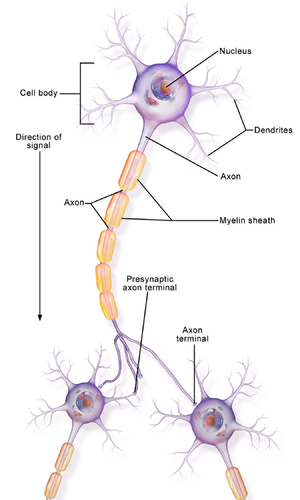
\includegraphics[width=0.25\textwidth]{figures/NeuronParts.png}
    \caption{A sketch of how a neuron may look like \cite{wiki:interneurons}}
    \label{fig:NeuronParts}
\end{wrapfigure}

In physiology, a neuron consists of a cell body or soma with the nucleus, dendrites and axon, as seen in the figure \ref{fig:NeuronParts}. The soma is a compact structure, whereas the axon and dendrites are filaments from the soma. Typically a dendrite receives signals from other neurons and the axon transmits information to other neurons. The cell body, soma, is where the nucleus lies and where proteins are made to be transported throughout the axon and dendrites.

A point where the distance between two neurons is lower than a certain threshold defines a touchpoint. If there is a touchpoint, then a synapse can emerge. A synapse is a structure that permits a neuron to pass an electrical or chemical signal to another neuron. There are different types of synapses. The most common is axodendritic. But there are also other types, depending on which parts of the neurons are in touch, such as axo-axonic (axon with axon), dendro-dendritic (dendrite with dendrite), axo-secretory (axon to bloodstream), somatodendritic (soma to dendrite), dendro-somatic (dendrite with soma), and somato-somatic (soma with soma) synapses. A neuron can have up to 6000 synapses with neighbouring neurons\cite{Sherwood2020}.

\section{Simulation of local neuronal network}
The usual workflow in research consists of three main steps: single-cell morphology reconstruction, building a local network and simulating the signals exchange.

The single-cell morphology reconstruction consists of retrieving the neurons' morphology to simulate. To do so, first, the bunch of neurons need to be separated to be able to do a reconstruction of the morphology of the neurons and a classification. Also, a repairing phase is necessary because there could have been errors in previous steps. This process ends up with isolated single-cell models. There are different databases with reconstructions of neuron morphologies, both private and public access, but the most common and huge is \href{https://neuromorpho.org/}{NeuroMorpho.Org} \cite{Neuromorpho1,Neuromorpho2}.

The network building step is computationally more intensive because there is a large number of points in the space where a lot of spatial calculations are involved. First, the single-cell models are cloned, transformed and translated to their final position. Then, all the touching points between the neurons need to be found. This task has a higher computational cost because it implies checking almost all the points of the neurons against all the compartments of the other neurons. Finally, the synapses are established according to geometric and biological restrictions.

Finally, simulating the signal exchange of the neurons relies on different software tools such as NEURON \cite{carnevale2006neuron}, Arbor \cite{8671560}, Brian \cite{Stimberg2019} and IBM Neural Tissue Simulator \cite{10.3389/fninf.2011.00015}. These programs allow the simulation of detailed biophysical models from single-cell models to large-scale networks.

\section{Space-partition data structures}
Space partitioning is the process of dividing a space into disjoint subsets, non-overlapping. The division can be done in two or more regions, and any point can then lie in only one subregion. Space partitioning is often hierarchical, which means the subsets are also divided recursively into other areas. The recursive division allows the organization of the subsets into a tree called a space-partitioning tree. 

The space-partitioning trees can divide the subsequent space into several regions each time or just two each iteration. When splitting the area into only two subregions, it is called binary space partitioning (BSP) tree. BSP trees usually use a hyperplane, a generalization of the plane for higher dimensions, to divide space, so the points on each side of the hyperplane form each subregion.

There is also another kind of tree that not only does it divides the space but also the time. For example, the TPR*-tree \cite{TPRtree}, but they are out of the scope of this thesis.

\subsection{Octree}
\begin{wrapfigure}{r}{0.5\textwidth}
    \centering
    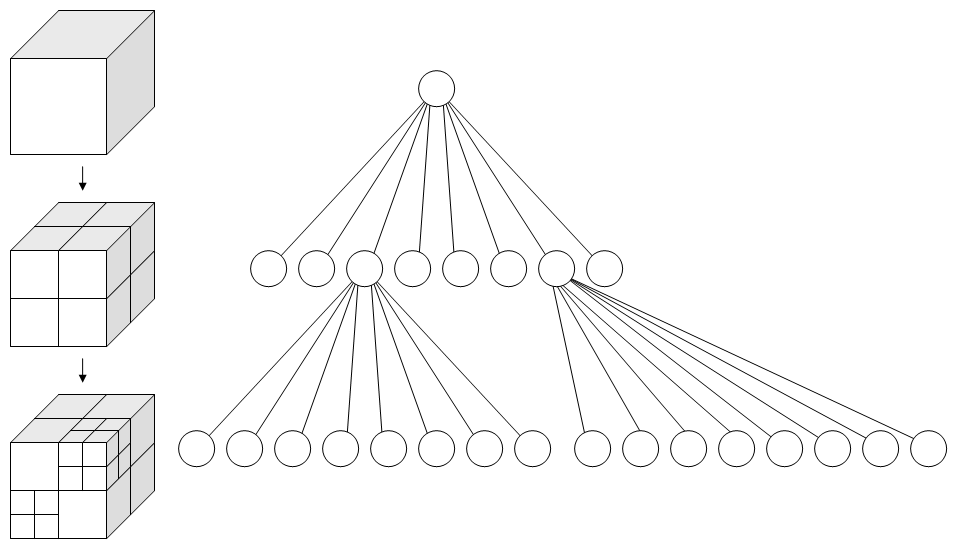
\includegraphics[width=0.5\textwidth]{figures/Octree.png}
    \caption{Left: Recursive subdivision of a cube into octants. Right: The corresponding octree. \cite{wiki:octree}}
    \label{fig:octree}
\end{wrapfigure}
An octree is a data structure to generate partitions of a 3D space. Each node has exactly eight children, except the leaves. There are two types of octree: point region (PR) octree and matrix-based (MX) octree. In a PR octree, the node represents one three-dimensional point, which is the centre of the subdivision, and it is one of the corners of the eight children. In an MX octree, the division point is implicitly the centre of the space. The root node of a PR octree represents infinite space, while in an MX octree, it represents a finite bounded space. When can see an example in the figure \ref{fig:octree}.

This data structure was proposed by Donald Meagher in 1980 \cite{Octree} and the construction goes as follows. First, it divides the current 3D volume into eight boxes. If any box has more than one point then apply again the algorithm. If the box has zero or one point, stop building that branch.

\subsubsection{Quadtree}
A quadtree is another tree data structure proposed earlier by Raphael Finkel and Joun Louis Bentley in 1974 \cite{Quadtree}. This data structure is the two-dimensional version of the Octree. Similar to the Octree, the algorithm divides the 2D space into four quadrants recursively. No more detail is needed for this data structure because our data is 3D-based and this solution works for 2D points.

\subsection{R-tree}
\begin{wrapfigure}{r}{0.5\textwidth}
    \centering
    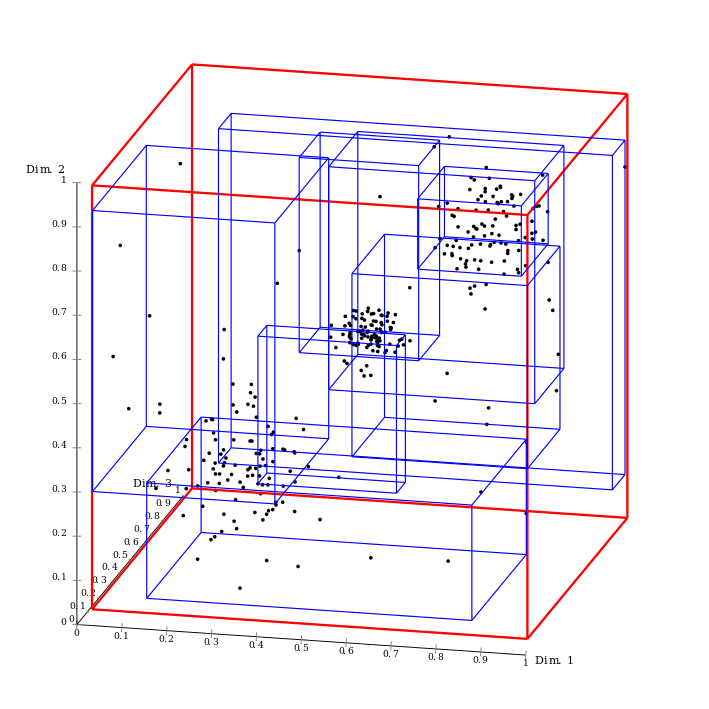
\includegraphics[width=0.5\textwidth]{figures/RTree-Visualization-3D.png}
    \caption{Visualization of an R*-tree for 3D points \cite{wiki:rtree}}
    \label{fig:rtree}
\end{wrapfigure}
An R-tree is a data structure used for spatial access methods for k-dimensional data. Antonin Guttman proposed the R-tree in 1984 \cite{10.1145/971697.602266} and the key idea is to group nearby points under a tight bounding box. The construction of the tree is button-up, which means the leaves are constructed first and it starts associating nodes with their bounding boxes until the root is reached. One visualization of the space partition made by an R-tree in a three-dimensional space can be seen in the figure \ref{fig:rtree}

This tree has different variations like priority R-tree, R$^*$-tree, R$^+$ tree, RR$^*$-tree, Hilbert R-tree and X-tree. One common variation used in the touching point problem is R*-tree. This variant has a slightly higher construction cost, but on the other hand, it will have a lower cost while querying. The main difference between R$^*$-tree and R-tree is that R$^*$-tree reduces the overlapping of subtrees, pruning more branches while querying and improving the performance, therefore. 

\pagebreak
\subsection{$k$-d trees}
\begin{wrapfigure}{r}{0.5\textwidth}
    \centering
    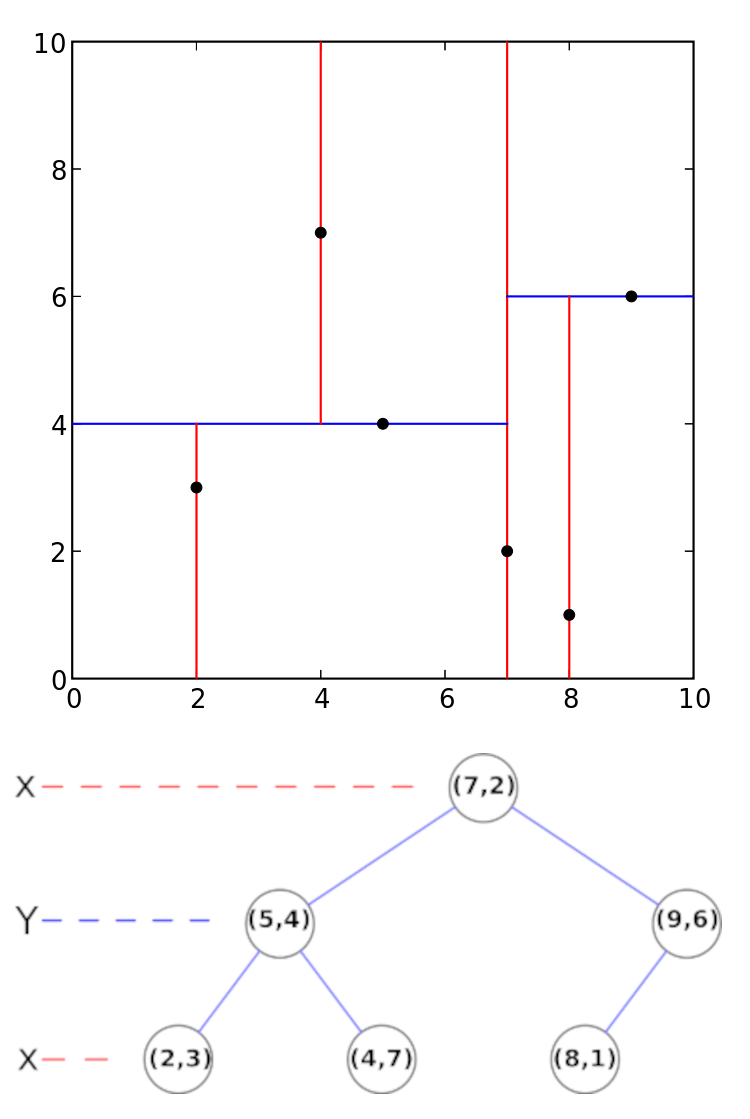
\includegraphics[width=0.5\textwidth]{figures/kdtree.png}
    \caption{k-d tree decomposition for a point set \cite{wiki:kdtree}}
    \label{fig:kdtree}
\end{wrapfigure}
$k$-d tree is a data structure for space-partitioning $k$-dimensional points. It is a characteristic case of space partitioning trees called binary space partitioning (BSP) trees. Being a BSP tree means that each time it splits the space it is done in two convex subsets. It was proposed in 1975 by Jon Louis Bentley \cite{Bentley}. The construction of the $k$-d tree is done recursively. First of all, one point and one axis are selected. Originally, the dimension was chosen by round-robin and the point was chosen by the median in that axis, but in this thesis, we will explore some other options. The axis and the point will form a hyperplane aligned with the axis. Then, the algorithm splits the points into two subsets: the point at the "left" of the plane and the points at the "right". Finally, the left and right subtrees are constructed using the same algorithm. One example of the execution of this algorithm can be seen in the figure \ref{fig:kdtree}.

\section{Previous research}
There are several studies on spatial-partitioning structures, but a little few focus on the touch detection problem. In their thesis, Adamsson and Vorkapic \cite{Adamsson_Vorkapic_2016} analyze the performance of different spatial-partitioning structures: $k$-d trees, vantage-point trees and octrees. They discovered that vantage-point trees are the best option with small populations, but $k$-d trees work better with larger networks. Because of their result, we choose $k$-d trees over other data structures. In Beredent and Brask's thesis \cite{Brask_Berendt_2020}, they analyze the memory efficiency for R-trees and R$^*$-trees. They analyzed the performance with realistic neuron densities and found out that R$^*$-tree has the same good scalability properties as $k$-d trees.

Compared with the studies on spatial-partitioning structures on the touch detection problem,  more studies are trying to optimize the $k$-d trees partition for different applications, such as computer graphics or curve analysis. Hu, Nooshabadi and Ahmadi in their paper \cite{LinjiaSaeidMajid} propose a method for constructing $k$-d trees and doing nearest neighbor search (NNS) with a speed up of a factor of 30, compared with a serial CPU. Wald and Havran \cite{WaldHavran06} propose an heuristic for choosing the dimension and splitting point called surface area heuristic that will speed up for raytracing with objects based on triangles. In other paper by different authors \cite{Yucheng}, they propose a heuristic called Curve Complexity Heuristic, which aim is to allow the exploration of 3D curves based on the neighbourhood.